\documentclass[a4paper]{article}

%% Language and font encodings
\usepackage[english]{babel}
\usepackage[utf8x]{inputenc}
\usepackage[T1]{fontenc}
\usepackage{xeCJK} 
%% Sets page size and margins
\usepackage[a4paper,top=3cm,bottom=2cm,left=3cm,right=3cm,marginparwidth=1.75cm]{geometry}
\usepackage{fontspec, xunicode, xltxtra}

%% Useful packages
\usepackage{amsmath}
\usepackage{graphicx}
\usepackage[colorinlistoftodos]{todonotes}
\usepackage[colorlinks=true, allcolors=blue]{hyperref}
\usepackage{listings}
\lstset{numbers=left, numberstyle=\tiny,basicstyle=\small, keywordstyle=\color{blue!70}, commentstyle=\color{red!50!green!50!blue!50}, frame=shadowbox, rulesepcolor=\color{red!20!green!20!blue!20},escapeinside=``, xleftmargin=2em,xrightmargin=2em, aboveskip=1em}

\begin{document}
% Titlepage & ToC
\hypersetup{pageanchor=false,
             bookmarksnumbered=true,
             pdfencoding=unicode
            }
\pagenumbering{roman}
\begin{titlepage}
\vspace*{7cm}
\begin{center}%
{\LARGE \textbf{Report of MOOC} }\\
\vskip 1cm

\includegraphics[width=1in]{Logo_ENSIIE.png}
\vskip 1cm
{\Huge \textbf{---------------------------------------------} }\\
\vskip 0.5cm
{\Huge \textbf{Machine Learning} }\\
\vskip 0.5cm
{\Huge \textbf{---------------------------------------------} }\\
\vskip 1cm
\vspace*{1cm}
{\large Guangyue CHEN}\\
\vspace*{0.5cm}
{\large{2018/12/12}}
\end{center}
\end{titlepage}
\tableofcontents{\LARGE}
\pagenumbering{arabic}
\hypersetup{pageanchor=true}


\newpage
\section{Introduction}
\Large{
	Machine learning is the science of getting computers to act without being explicitly programmed. It involves many machine learning algorithms, which is a kind of automatic analy- sis from the data to obtain the law, and use the law of the algorithm to predict the unknown data. Because the learning algorithm involves a lot of statistical theory, ma- chine learning and inferred statistics are particularly close, also known as statistical learning theory.
\subsection{Machine Learning - Coursera}
This Stanford online courses is taught by Andrew Ng who is one of the mostly influencing professors in Machine Learning. In this class,  l learned about not only the theoretical underpinnings of learning, but also gain the practical know-how needed to quickly and powerfully apply these techniques to new problems. Finally, I realized some of Silicon Valley's best practices in innovation as it pertains to machine learning and AI.


\section{Course content}
The course has a total of 11 weeks. In each week, it introduces us to the common ma- chine learning model and principle of algorithm, which also involves some derivations of mathematical formula. It has the test every weak. What's more, it has also one project per week to practice the knowledge that we learned. In general, it is divided into the following sections.
\subsection{Supervised learning}
In supervised learning, we are given a data set and already know what our correct output should look like, having the idea that there is a relationship between the input and the output.\\
\subsubsection{\textbf{Linear Regression}}
In the linear regression model, through the feature extraction, we rst select the char-acteristic variable x which a ects the estimated variable y, and then through our train- ing set and learning algorithm, we can get a hypothesis h. Here h can Be expressed as:$$h_\theta(x)=\theta_0+\theta_1*x_1+\theta_2*x_2+...$$
Here We measure the accuracy of our hypothesis function by using a cost function $J(\theta)$.$$Cost function: J(\theta)=-\frac{1}{2m}\sum_{i=1}^{m}(h_\theta(x^{(i)})-y^{(i)})$$ Then we choose the parameters who minimize the cost function. the main method optimized we used is \textbf{Gradient Descent} which is:\\repeat until convergence$$\theta_j=\theta_j-\alpha\frac{1}{m}((h_\theta(x^{(i)})-y^{(i)})*x_j^{(i)}$$where m is the number of the observations and $\alpha$ is the learning rate which we should choose by ourselves. It \\
\textbf{\href{https://github.com/GuangYueCHEN/ENSIIE/tree/master/Plus/MachineLearning/machine-learning-ex1}{practice:ex1} }\\
\begin{center}
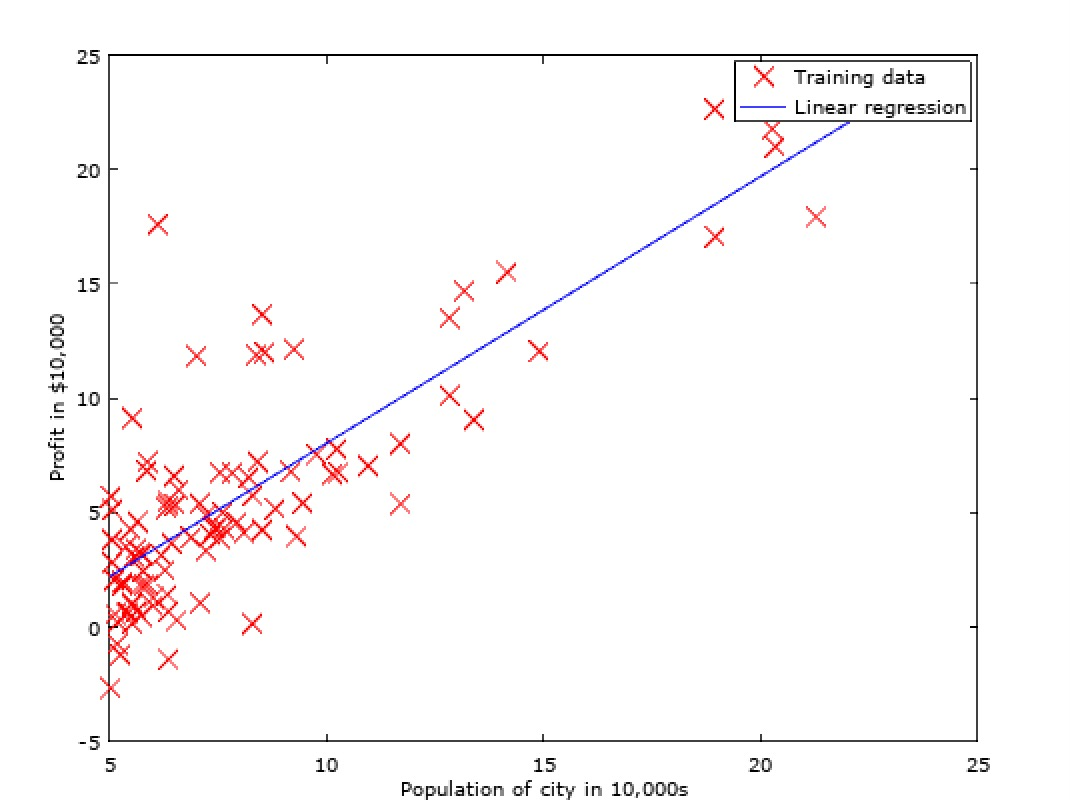
\includegraphics[width=3in]{linear.png}\\
Figure1:The result of Linear Regression
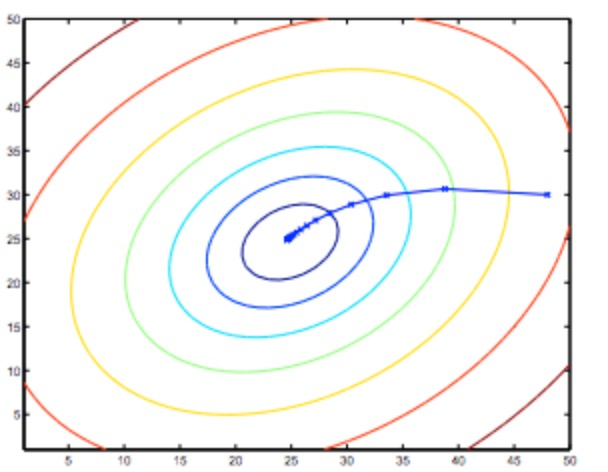
\includegraphics[width=3in]{grad.png}\\
Figure1:The converge of Gradient Descent
\end{center}
\subsubsection{\textbf{Logistic Regression}}
The classification problem is just like the regression problem, except that the values we now want to predict take on only a small number of discrete values. And here one inportant thing is to dicide the \textbf{decision boundary}$$h_\theta(x)\ge0.5,y=1.$$
	$$h_\theta(x)<0.5,y=0.$$
Furthermore, with vectoration, we get:$$h_\theta(x)=g(\theta^Tx)\ge0.5$$$$when:\theta^Tx\ge0$$\\We cannot use the same cost function that we use for linear regression because the Logistic Function will cause the output to be wavy, causing many local optima. In other words, it will not be a convex function.

Considering y equals 0 or 1, our cost function for logistic regression looks like:$$J(\theta)=-\frac{1}{m}\sum_{i=1}^m[y^{(i)}log(h_\theta(x^{(i)}))+(1-y^{(i)})log(1-h_\theta(x^{(i)}))]$$
Here we use the octave's "fminunc()" optimization algorithm along with the "optimset()" function that creates an object containing the options we want to send to "fminunc()".
\begin{lstlisting}[language=Octave]
%  Set options for fminunc:
options = optimset('GradObj', 'on', 'MaxIter', 400);

%  Run fminunc to obtain the optimal theta
%  This function will return theta and the cost 
[theta, cost] = ...
	fminunc(@(t)(costFunction(t, X, y)), initial_theta, options);

\end{lstlisting}
Le code completet: \href{https://github.com/GuangYueCHEN/ENSIIE/tree/master/Plus/MachineLearning/machine-learning-ex2}{Logistic}.
\newpage
\begin{center}
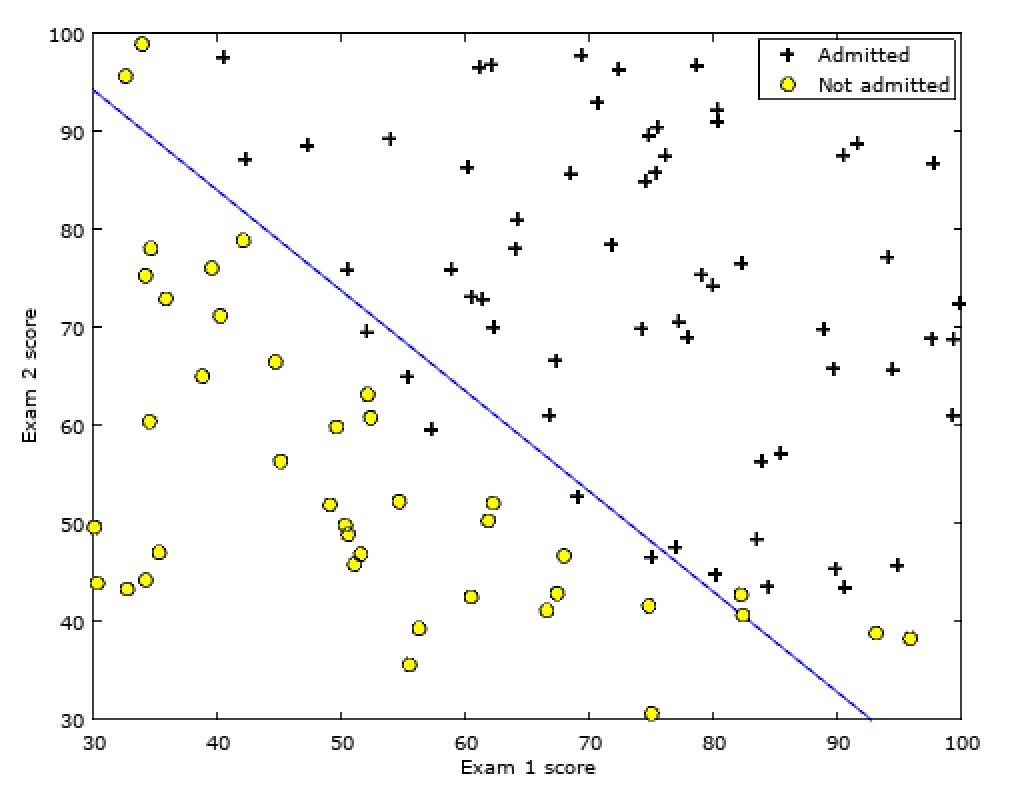
\includegraphics[width=3in]{log.png}\\
Figure3:The result of Logistic Regression
\end{center}
\subsubsection{\textbf{Regularization}}
 Consider the problem of Overfitting, we add the regularization. So we could aregularize all of our theta parameters in a single summation as$$J(\theta)=-\frac{1}{2m}\sum_{i=1}^{m}(h_\theta(x^{(i)})-y^{(i)})+\lambda\sum_{j=1}^n\theta_j^2$$
The $\lambda$ is the regularization parameter. It determines how much the costs of our theta parameters are inflated.
Regularization is used in many projects of this course.
\subsubsection{\textbf{Multi-class Classification and Neural Networks}}
To classify data into multiple classes, we let our hypothesis function return a vector of values. Here we use the model \textbf{"Neural Networks"} the method \textbf{"Backpropagation"}.
\begin{center}
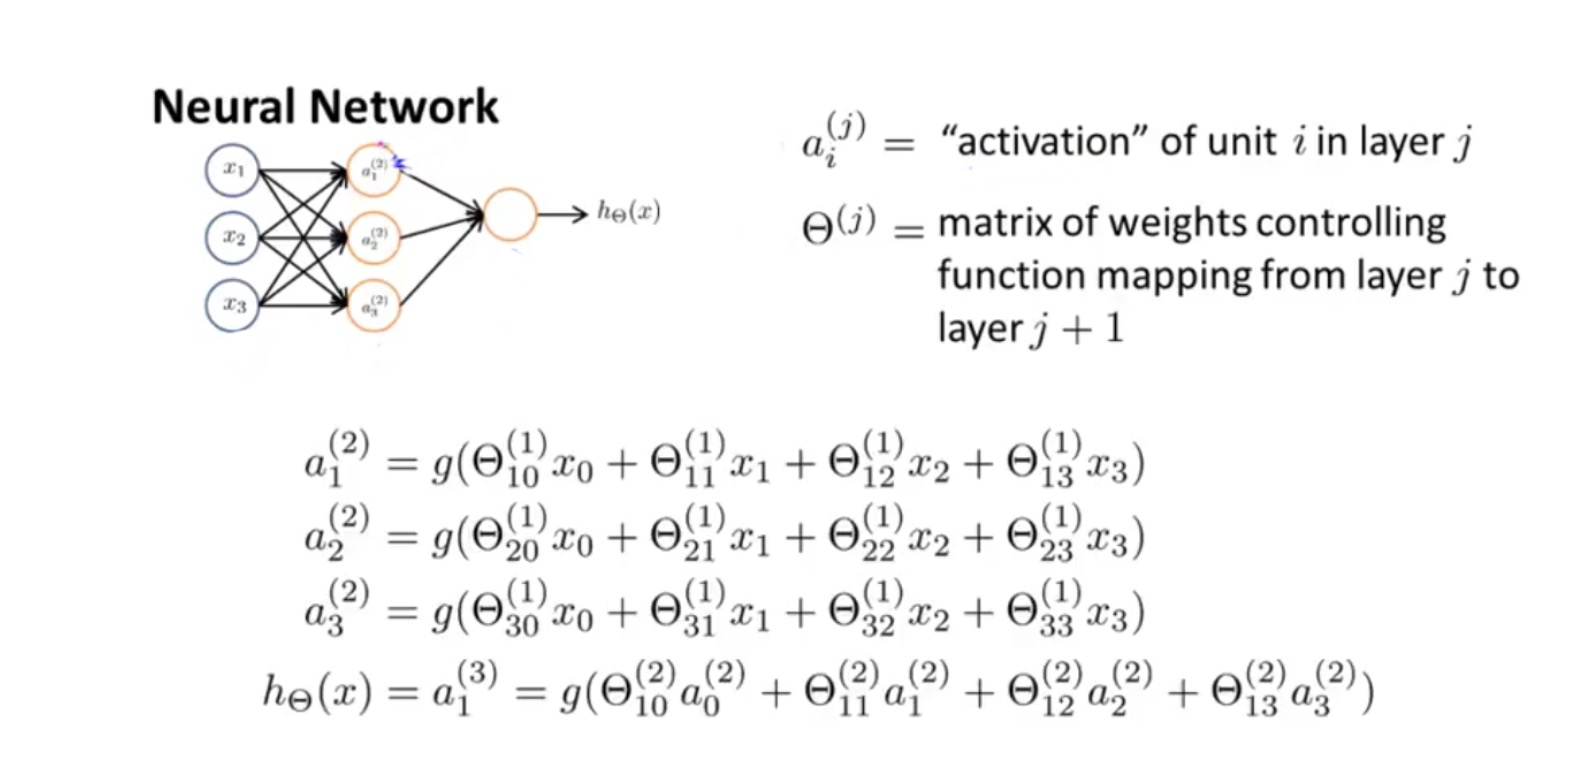
\includegraphics[width=5in]{nn.png}\\
Figure4:Neural Networks Model
\end{center}
In the \textbf{Neural Networks} model, there are 3 types of layer: input layer, hidden layer, output layer. Each layer content n nodes. After the modelization, we can compute our activation nodes by using a matrix of parameters. We apply each row of the parameters to our inputs to obtain the value for one activation node.\\
\begin{center}
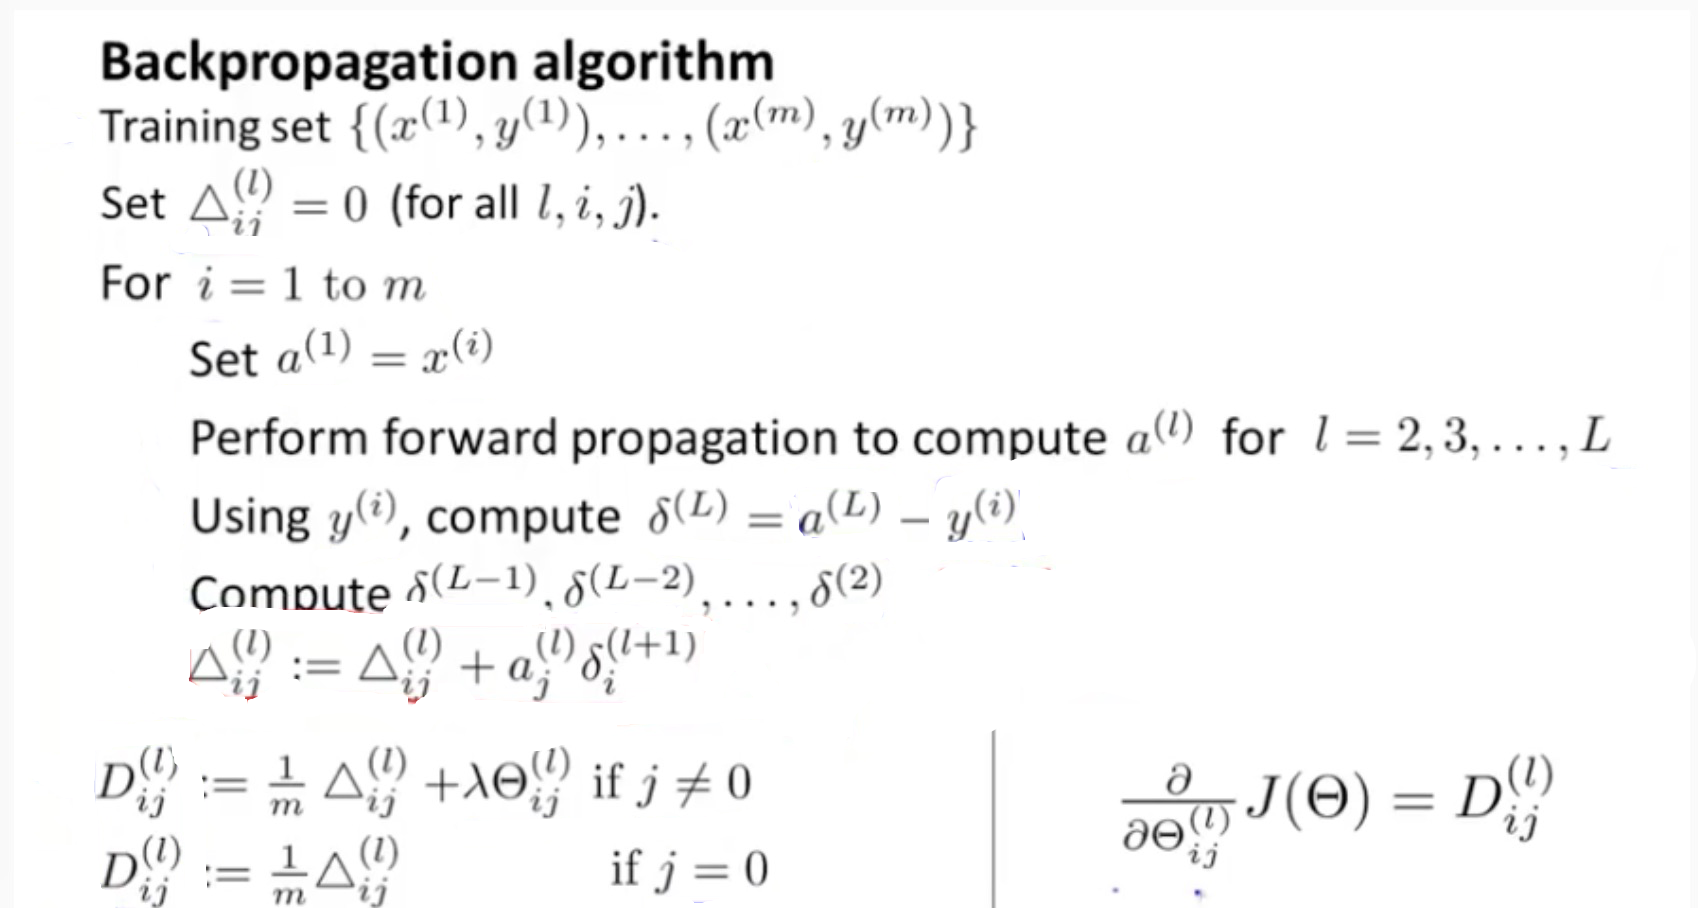
\includegraphics[width=5in]{back.png}\\
Figure5:Backpropagation Algorithm
\end{center}
\textbf{"Backpropagation"} is neural-network terminology for minimizing our cost function, just like what we were doing with gradient descent in logistic and linear regression. 

Then we do the most important project, we implement the backpropagation algorithm for neural networks and apply it to the task of hand-written digit recognition.

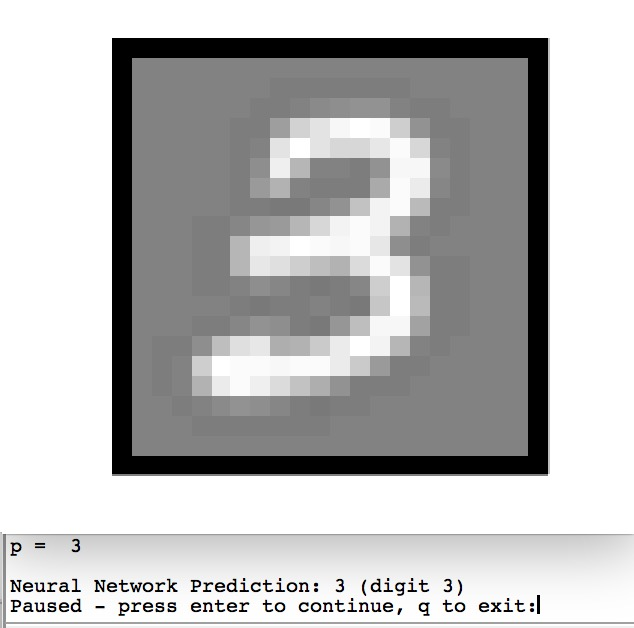
\includegraphics[width=2in]{3.png}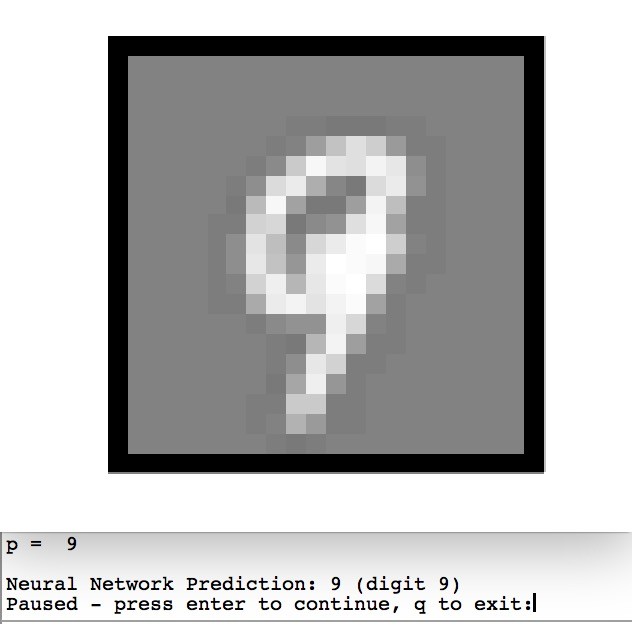
\includegraphics[width=2in]{9.png}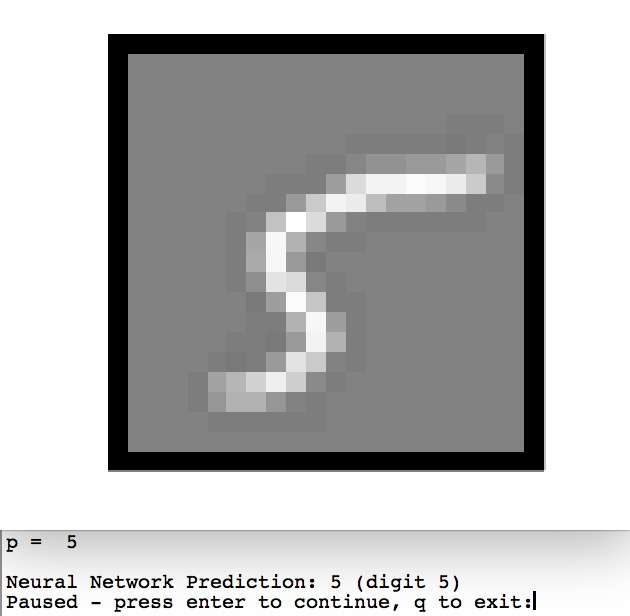
\includegraphics[width=2in]{5.png}
\begin{center}
Figure6:The result
\end{center}
\href{https://github.com/GuangYueCHEN/ENSIIE/tree/master/Plus/MachineLearning/machine-learning-ex3}{All code here}.\\
\subsubsection{\textbf{Support Vector Machines}}
  There's one more algorithm that is very powerful and is very widely used both within industry and academia, and that's called the support vector machine. SVM gives a cleaner, and sometimes more powerful way of learning complex non-linear functions.
 $$min_\theta C\sum_{i=1}^m[y^{(i)}cost_1(\theta^Tx^{(i)})+(1-y^{(i)})cost_0(\theta^Tx^{(i)})]+\frac{1}{2}\sum_{j=1}^n\theta^2_j$$$$where:cost_1(\theta^Tx^{(i)})=-logh_\theta(x^{(i)})$$$$cost_0(\theta^Tx^{(i)})=-log(1-h_\theta(x^{(i)}))$$
 
 So we want :
 
 If y = 1, we want $ \theta^Tx\ge 1$,
 and if y = 0, we want $\theta^Tx\le -1$. It will give us a large \textbf{Decision Boundry}. Here we have a project too.
\href{https://github.com/GuangYueCHEN/ENSIIE/tree/master/Plus/MachineLearning/machine-learning-ex6}{All code here}.\\
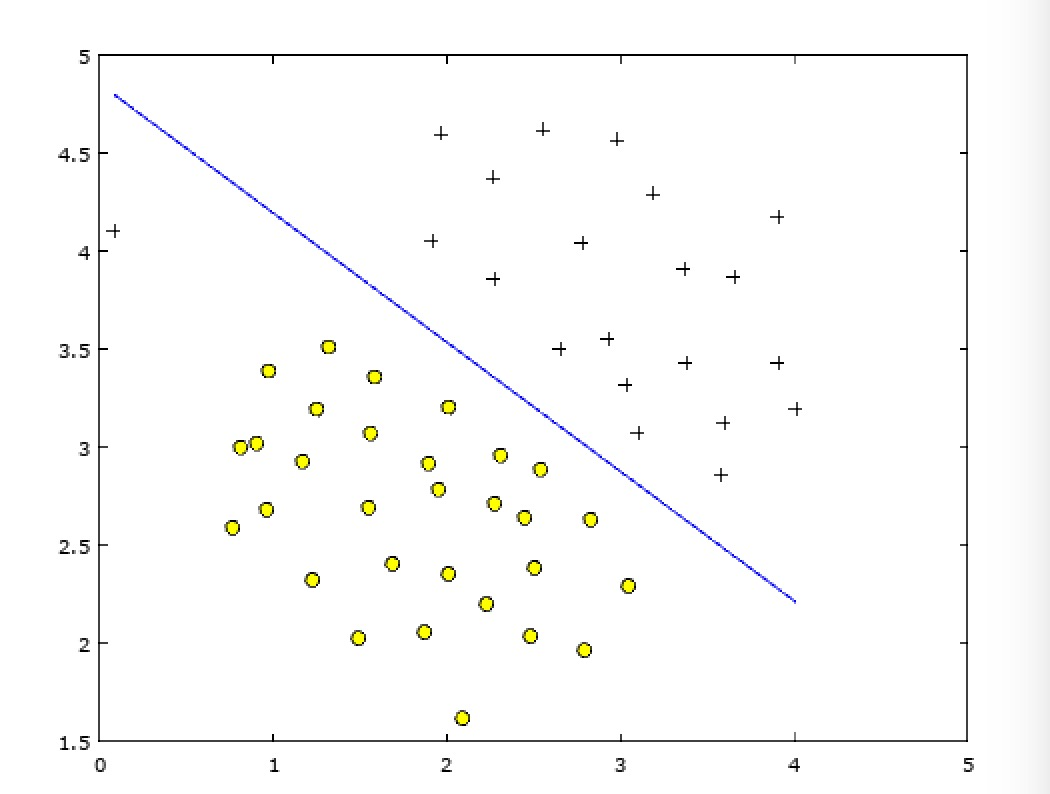
\includegraphics[width=3in]{svm2.png}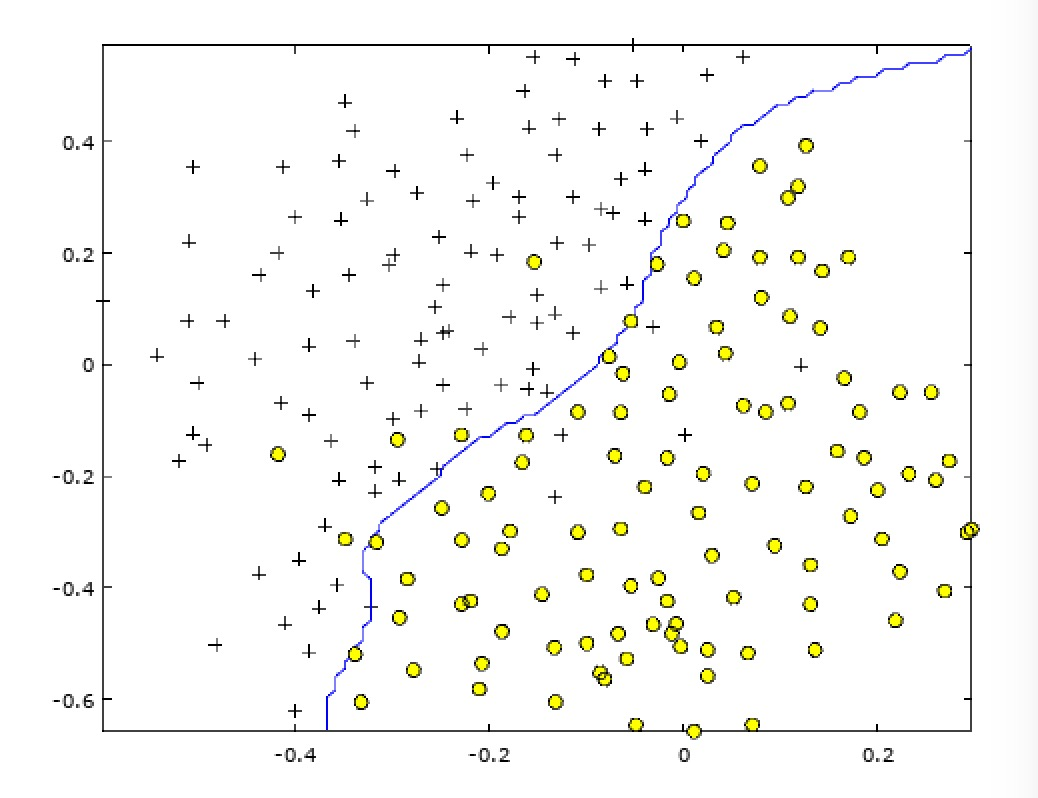
\includegraphics[width=3in]{svm.png}
\begin{center}
Figure7:Decision Boundry made by SVM
\end{center}
So we can see the higher standard conditions make the SVM get the largest Margin’s decision boundary.




\subsection{Unsupervised learning}
In supervised learning, we are given a data set and already know what our correct output should look like, having the idea that there is a relationship between the input and the output.\\
\subsubsection{\textbf{Principal Component Analysis}}
PCA is an unsupervised linear dimensionality reduction algorithm to find a more meaningful basis or coordinate system for our data and works based on covariance matrix to find the strongest features if your samples. So what PCA does formally is it tries to find a lower dimensional surface onto which to project the data so that the sum of squares of variance is minimized.

We have learnt many knowledge about PCA, PCoA and KPCA from the course `MAD',  which teach us more things.  But this course spend more at practice. So I gain that  PCA can help us to Reduce memory/disk needed to store data. And speed up learning algorithm.
\subsubsection{\textbf{K-Means Clustering}}
K-means clustering is a type of unsupervised learning, which is used when we have unlabeled data. The goal of this algorithm is to find groups in the data, with the number of groups represented by the variable K. The algorithm works iteratively to assign each data point to one of K groups based on the distances between the data points and the group centers.
\begin{center}
\textbf{K-means algorithm}\\
\end{center}
Randomly initialize K cluster centroids $\mu_1,\mu_2,...,\mu_k$\\
Repeat\{\\
for i = 1 to m\\
	$c^{(i)}$:= index(from 1 to K) of cluster centroid closest to $x^{(i)}$\\
for k = 1 to m\\
		$\mu_k$:= average(mean) of points assigned to cluster k\\
	\}\\
 Project:
 \begin{center}
 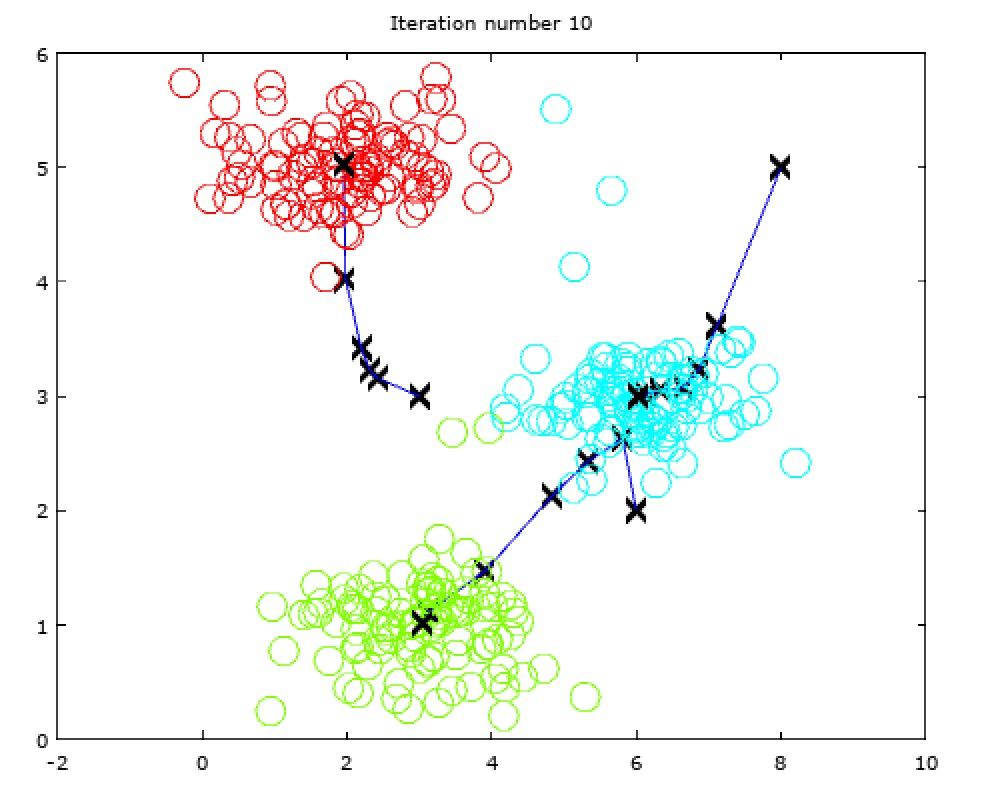
\includegraphics[width=5in]{kmean.png}
Figure8:Iteration of K-means
\end{center}
So we can see with the ieration, the centroids is closer to the center of real class. 
\href{https://github.com/GuangYueCHEN/ENSIIE/tree/master/Plus/MachineLearning/machine-learning-ex7}{All code here}.\\
\subsection{Best practices in machine learning}
\subsubsection{\textbf{Anomaly Detection}}
For this part, the teacher modelize the real problem into the mixture model. With eht estimation of the distribution, we can evidently know which object or which user is anomaly.\\
\textbf{Anomaly Detection}\\
1. Choose features $x_i$ which might be indicative of anomalous examples.\\
2. Fit parameters $\mu_1,\mu_2,...,\mu_n,\sigma_1,\sigma2,...,\sigma_n$\\
$$\mu_j=\frac{1}{m}\sum_{i=1}^{m}x_j^{(i)}$$
$$\sigma_j^2=\frac{1}{m}\sum_{i=1}^{m}(x_j^{(i)}-\mu_j)^2$$\\
3. Given new example x, compute $p(x)$:
$$p(x)=\Pi_{j=1}^np(x_j;\mu_j;\sigma_j^2)=\Pi_{j=1}^n\frac{1}{\sqrt[]{2\pi}\sigma_j}exp(1\frac{(x_j-\mu_j)^2}{2\sigma_j^2})$$\\
4. Anomaly if p(x) < $\varepsilon$.
 \begin{center}
 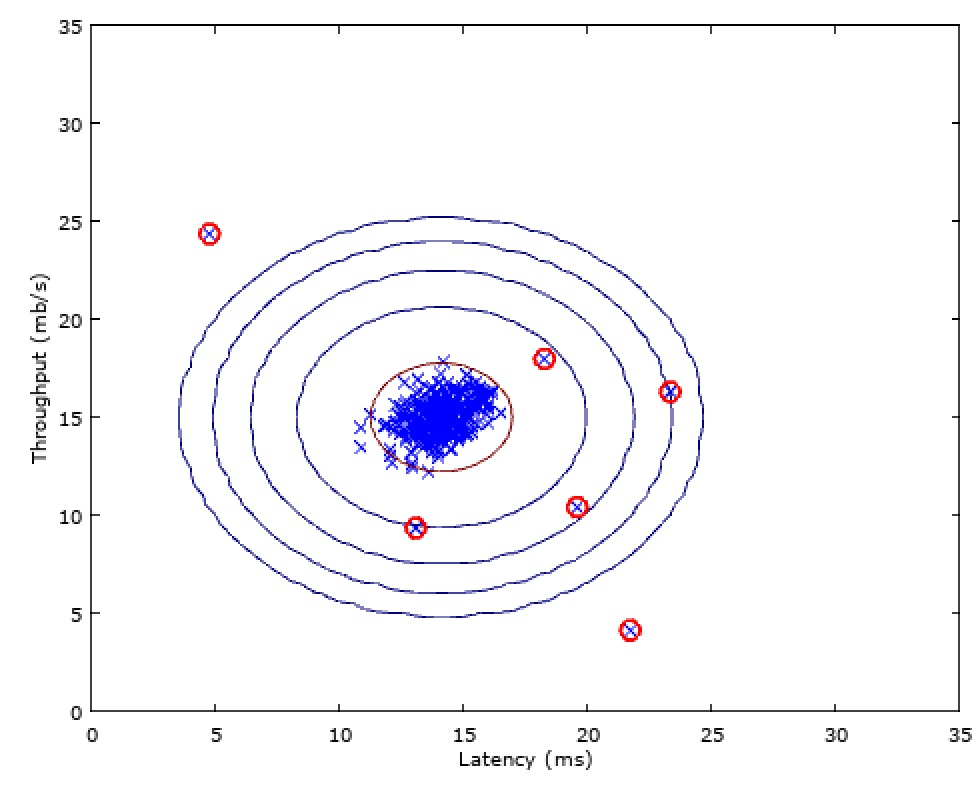
\includegraphics[width=5in]{dt.png}
Figure8:Anomaly Detection
\end{center}
\subsubsection{\textbf{Recommender Systems}}

The recommender systems is an important application of supervised machine learning. So we can recommender users the movies or the novels after they rate the same kinds movies or novels. Here the main conception is \textbf{Collaborative Filtering}. The system learn better features and then these features can be used by the system to make better movie predictions for everyone else. And also every user is helping the system learn better features for the common good when they rate new movies. 
\subsubsection{\textbf{Application: Photo OCR}}
This part is just the introduction of one popular machine learning technology: Photo Optical Character Recognition, or OCR.  It can convert the photo into editable data. We can use the \textbf{Sliding windows} to do the \textbf{Text detection} or \textbf{Pedestrian  detection}.

\subsection{Tool and Language}
\textbf{Octave}\\
The Octave syntax is largely compatible with Matlab. The Octave interpreter can be run in GUI mode, as a console, or invoked as part of a shell script. Here all the projects are written in Octave.

\newpage
\section{Conclusion}
After a period of study, I learned about the most effective machine learning techniques, and gain practice implementing them and getting them to work for myself. It helps me to gain deeper and more various machine learning models and algorithms which is useful to be a data scientist. To conclusion, I benefit a lot from this course.
}
\section{Appendix}
\subsection{Course and Github}

Course:\href{https://www.coursera.org/learn/machine-learning/}{https://www.coursera.org/learn/machine-learning/} \\
Github(all 7 projects):\href{https://github.com/GuangYueCHEN/ENSIIE/tree/master/Plus/MachineLearning}{https://github.com/GuangYueCHEN/ENSIIE/MachineLearning} 

\subsection{progress}
After 11 weeks studying, I passed this course. My final resault is 96/100.
\begin{center}
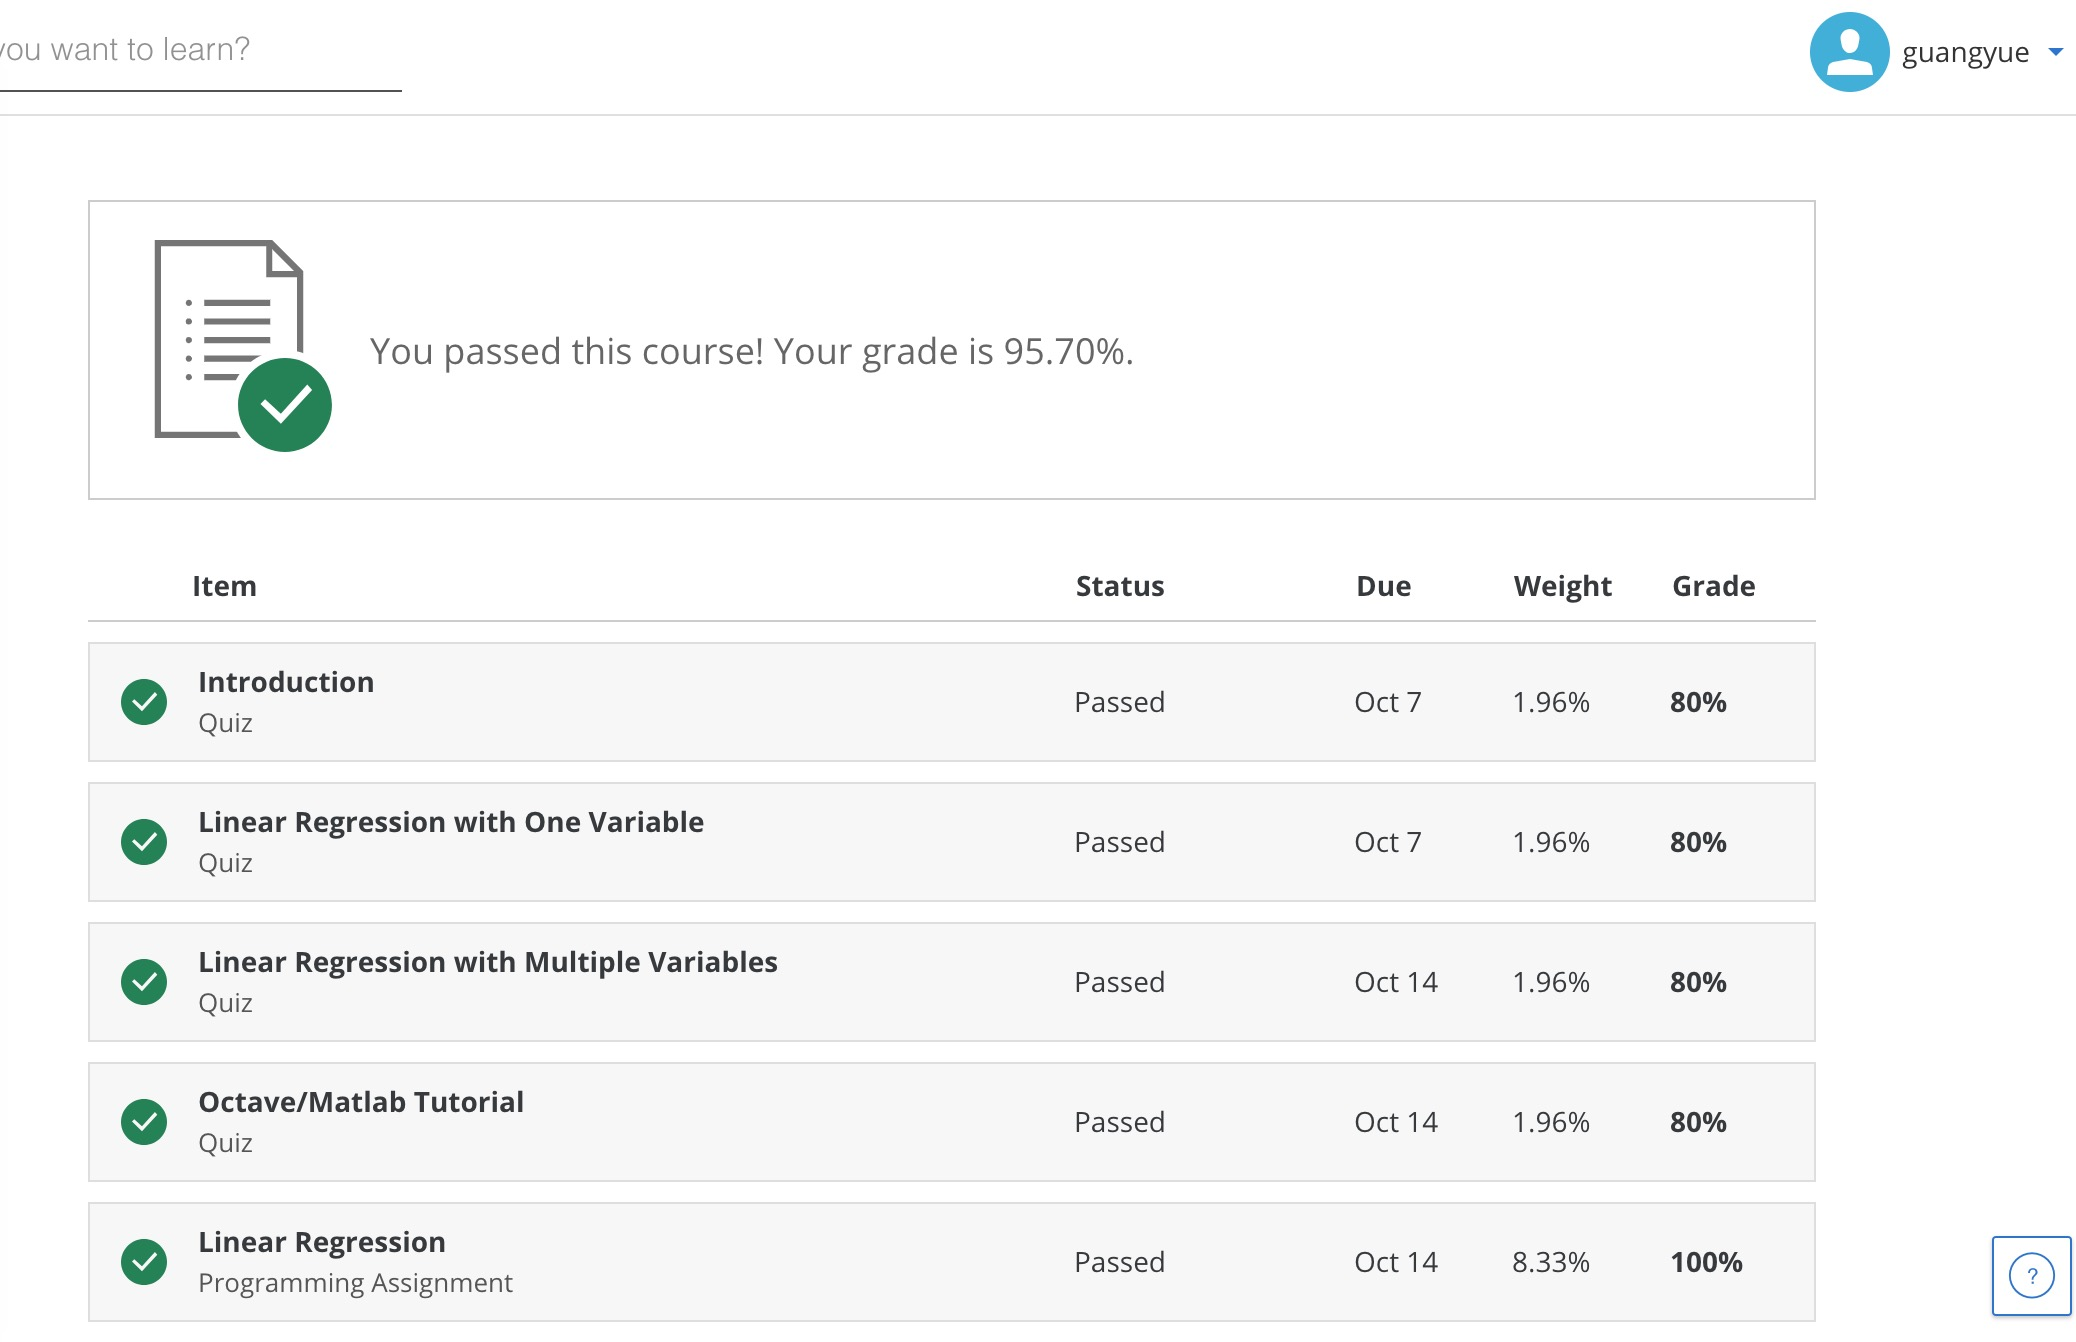
\includegraphics[width=5in]{res1.png}
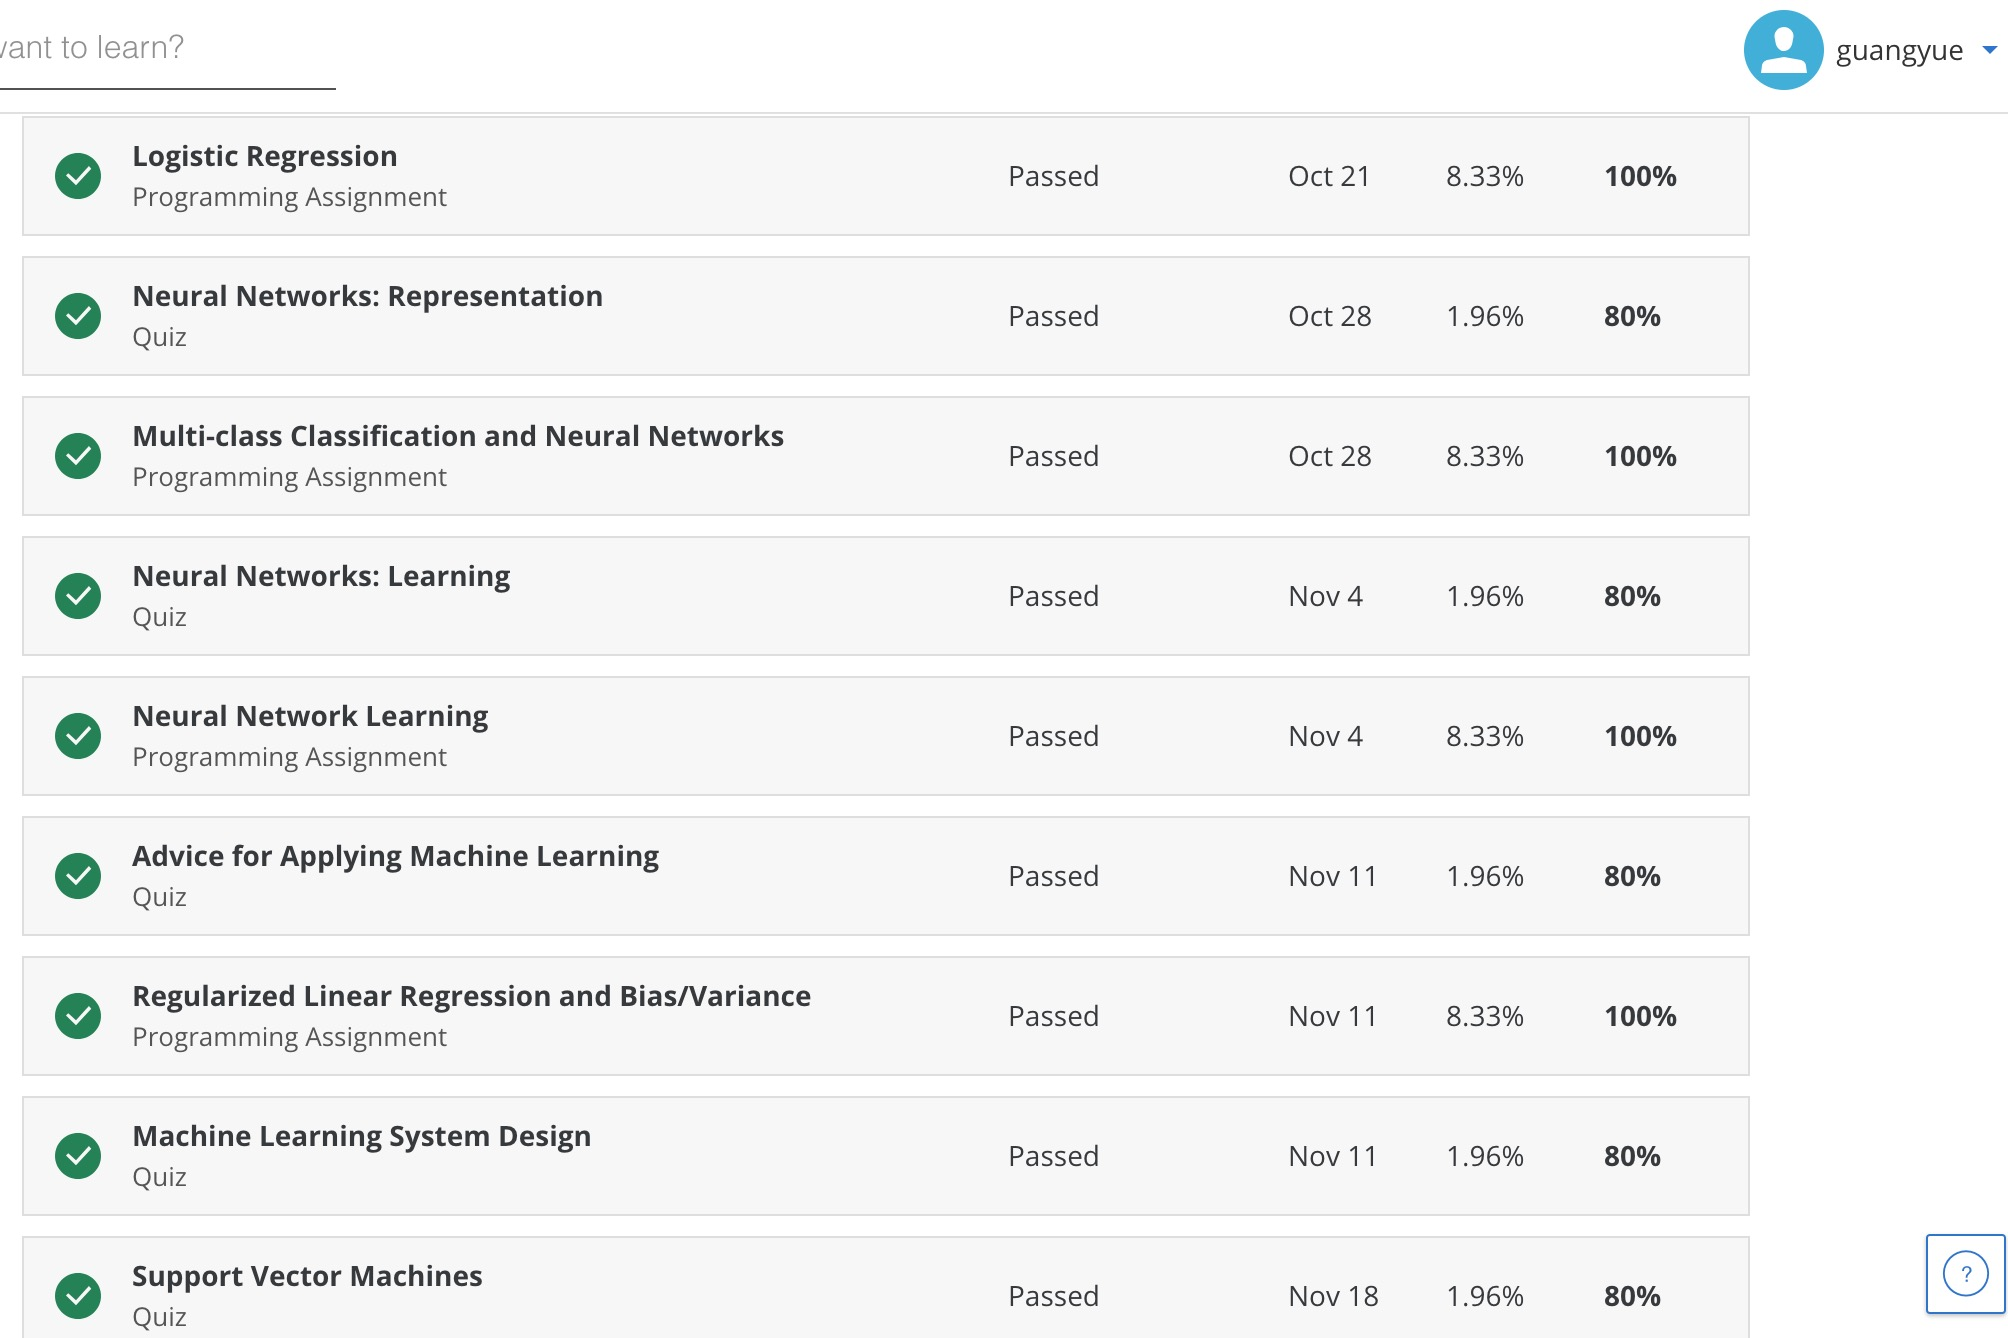
\includegraphics[width=5in]{res2.png}
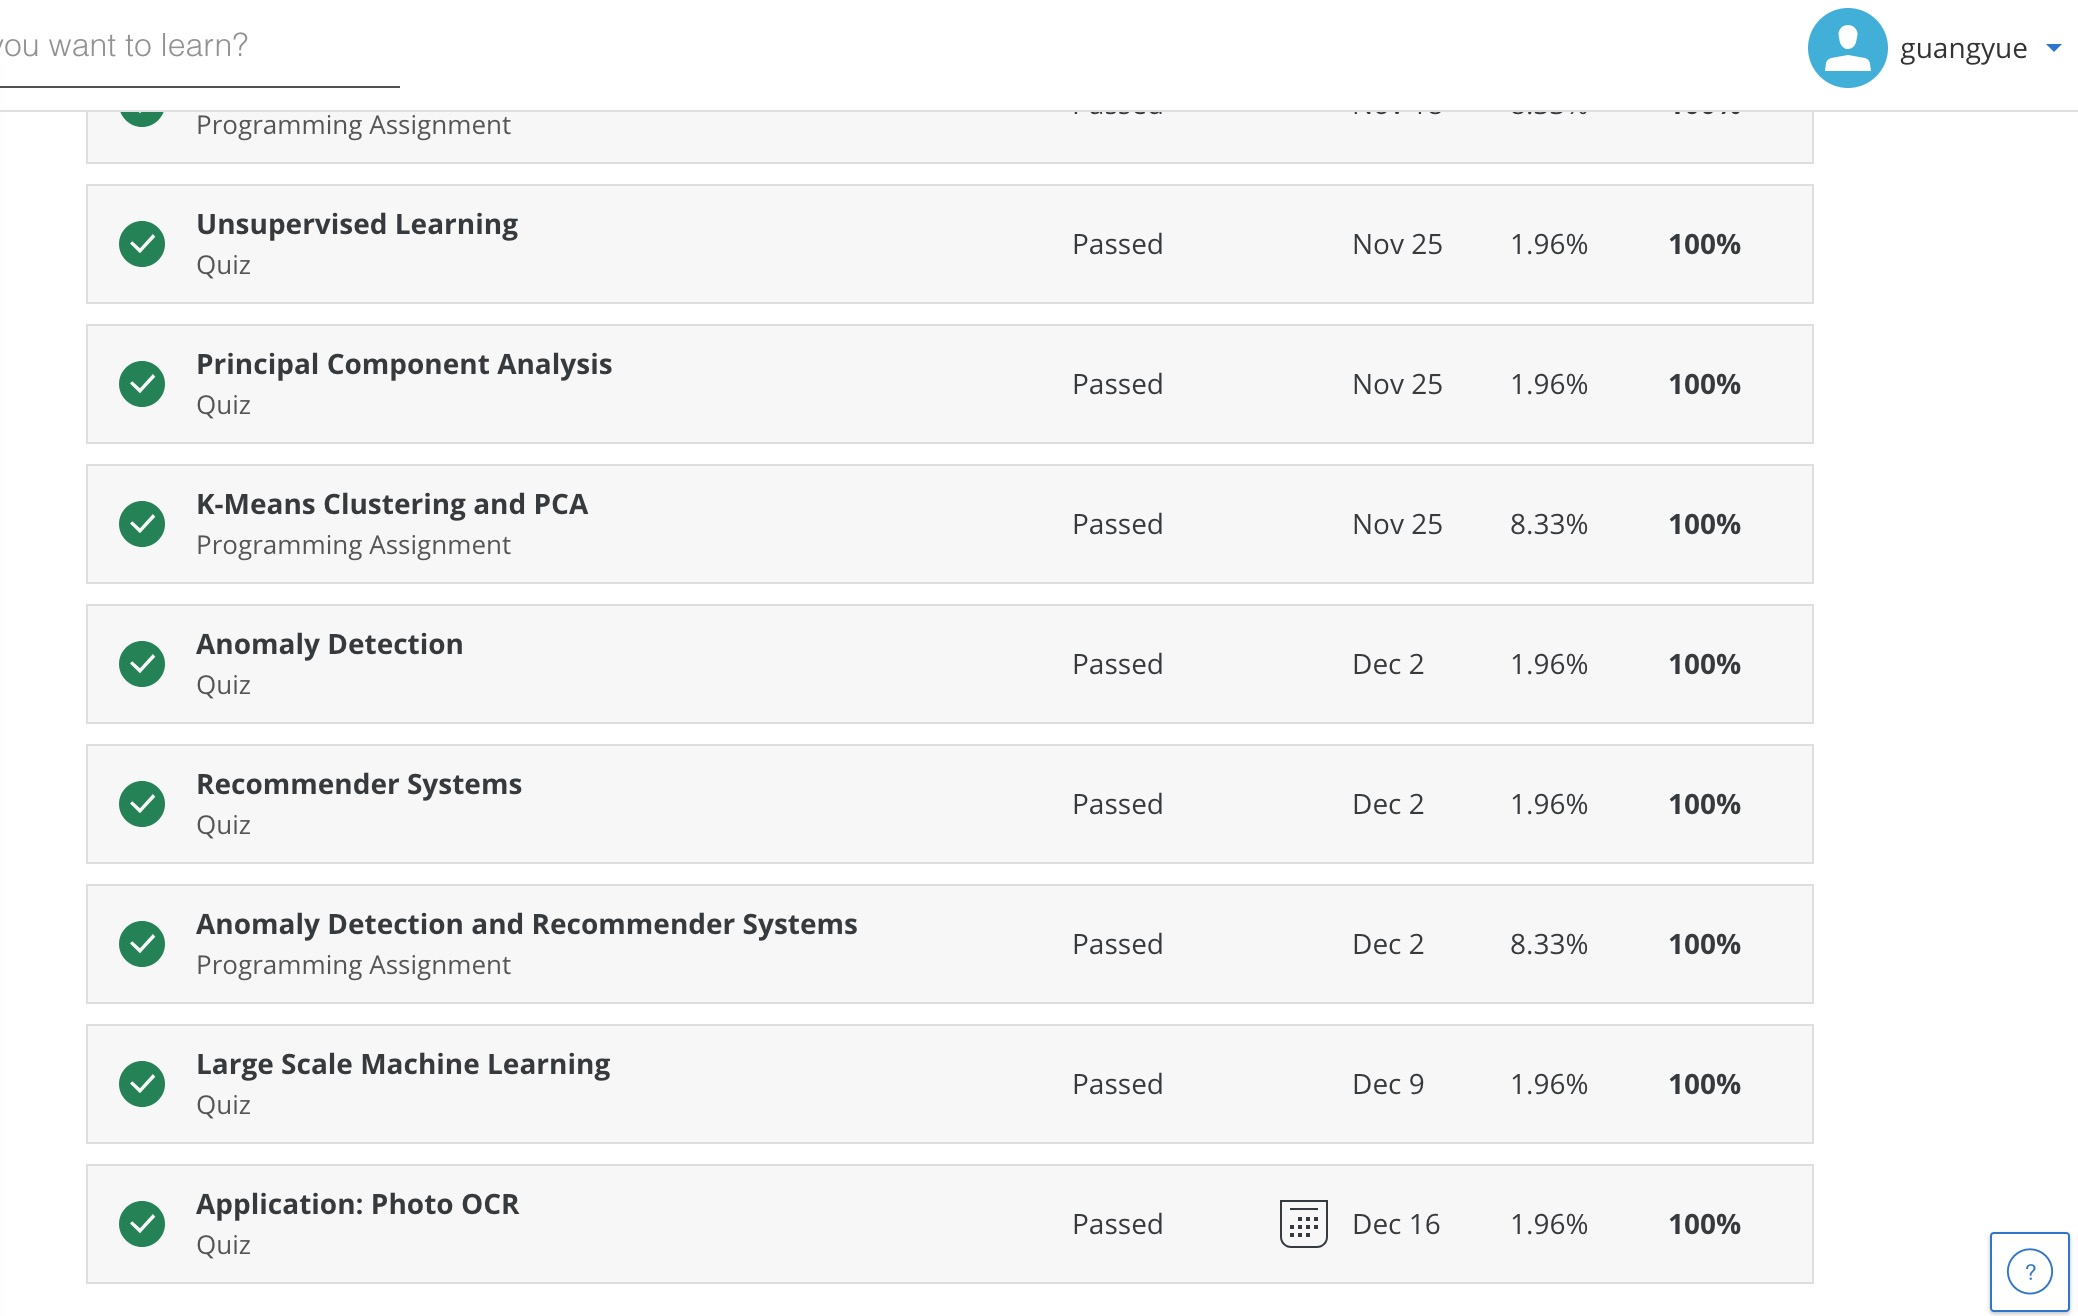
\includegraphics[width=5in]{res3.png}
\end{center}
\end{document}